% This is a template for doing homework assignments in LaTeX

\documentclass{article} % This command is used to set the type of document you are working on such as an article, book, or presenation

\usepackage[margin=1in]{geometry} % This package allows the editing of the page layout
\usepackage{amsmath}  % This package allows the use of a large range of mathematical formula, commands, and symbols
\usepackage{graphicx}  % This package allows the importing of images
\usepackage{amsfonts}
\usepackage{enumitem}
\usepackage{listings}
\usepackage{hyperref}

% \setlength\parindent{0pt}

\newcommand{\question}[2][]{\begin{flushleft}
                                \textbf{Question #1}: \textit{#2}

\end{flushleft}}
\newcommand{\sol}{\textbf{Solution}:} %Use if you want a boldface solution line
\newcommand{\maketitletwo}[2][]{\begin{center}
                                    \Large{\textbf{Project #1}

                                    ICCS315: Applied Algorithms} % Name of course here
                                    \vspace{5pt}

                                    \normalsize{Thanatad Anukoolprasert, Yuttasart Viratpan   % Your name here

                                    \today}        % Change to due date if preferred
                                    \vspace{15pt}
\end{center}}
\begin{document}
    \maketitletwo[]  % Optional argument is assignment number
    %Keep a blank space between maketitletwo and \question[1]

    \section*{Objective}
    The objective of this project is to benchmark two different type of data structures and compare different
    implementation of each type as well as their theoretical running time.
    The first type is resizable array where the following data structures are of interest
    \begin{itemize}
        \item Hashed Array Tree (Sitarski, 1996)
        \item Brodnik's resizable array non-superblock version (Brodnik et al., 1999)
        \item Brodnik's resizeable array superblock version (Brodnik et al., 1999)
    \end{itemize}

    The second type is hash table with 3 different collision resolution schemes, namely
    \begin{itemize}
        \item Chaining
        \item Open addressing
        \item Cuckoo hashing (Rasmus Pagh \& Flemming Rodler., 2004)
    \end{itemize}

    For a lack of a better name, we are going to called both the data structures from \href{ https://sedgewick.io/wp-content/themes/sedgewick/papers/1999Optimal.pdf}{ Brodnik et al 1999}, Hashed Array Tree (HAT).
    Not only that we are going to called Brodnik's HAT with non-superblock version \emph{Brodnik's HAT A} and the superblock version \emph{Brodnik's HAT B}.

    The dimensions of interest are the following
    \begin{itemize}
        \item Append latency
        \item Access latency
        \item Scan throughput
        \item Overall throughput
    \end{itemize}

    \section*{Method}
    We are going the implement the data structures above and benchmark them. Our implementation can be found here: \href{https://github.com/thanatadcs/apal-project}{ https://github.com/thanatadcs/apal-project}.
    We are going the measure running time in cycles using
    \emph{rdtsc} assembly instruction in x86 so that we are able to time quick operation like append with accurary.

    \subsection*{Remark on implementation}
    The implementation of \emph{get} function of Brodnik's HAT B is different from \emph{locate} function in the original paper.
    Namely, we cannot implement part of \emph{locate} function since there might be something wrong with the pseudocode in the paper,
    specifically \emph{$p=2^k - 1$} mentioned in the paper does not represent the number of data blocks before the $k$-th superblock as claimed,
    but it represent the number of elements before the $k$-th superblock instead. For this reason I have to implement my own way to get the number of
    data blocks before the $k$-th superblock. This can effect the running time of the \emph{get} function for Brodnik's HAT B. More information can be found in brodnik-hat-b.cpp.

    For Brodnik's HAT A and B, background-rebuilding optimization are also implemented so that we get $O(1)$ worst case append time. Brodnik's HAT B also utilized BSR assembly instruction in x86 to find
    the superblock number.

    \section*{Results and Discussion}
    \subsection*{Hashed Array Tree}
    All the number presented has the unit in cycles.
    \subsubsection*{Append latency}
    10 millions elements are appended and each append are timed, here are the statistics
    \begin{center}
        \begin{tabular}{|c|c|c|c|}\hline
        & Sitarski's HAT & Brodnik's HAT A & Brodnik's HAT B\\\hline
        mean &  59.7470848 & 48.3077336 & 46.6222048\\\hline
        standard deviation & 28458.271801239895  & 173.0441420332727 & 227.73642714240262\\\hline
        \end{tabular}
    \end{center}
    For append latency, the ranking from best to worst running time is Brodnik's HAT B, Brodnik's HAT A, and Sitarski's HAT.
    This makes sense since Sitarski's HAT have to copy not only the pointer, but also all elements every time it's expand as compare to Brodnik's HAT A
    and B where only pointer need to be copy and since we do not need to copy the elements, background-rebuilding is possible which make this even better and in fact constant in term of append time.

    In another aspect, our results also follow the theoretical running time very well. For Sitarski's HAT, in theory append time is $O(1)$ amortized, so we can see that the mean
    is that not far off from Brodnik's A and B, but since this is amortized cost, the standard deviation can be very high since there might be spike in running time once in a while. Brodnik's A and B has $O(1)$ worst case append time so
    the standard deviation of both of these is very low. Here is a the plot for append time
    \begin{center}
        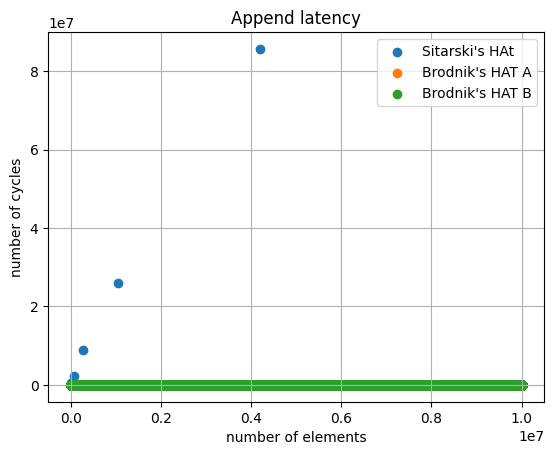
\includegraphics{graphics/hat_append.png}
    \end{center}
    which demostrated how the append time for Brodnik's A and B are constant.
    \subsubsection*{Access latency}
    10 millions elements are appended and all 10 millions elements get access through \emph{get} function.
    Each access is timed, here are the statistics
    \begin{center}
        \begin{tabular}{|c|c|c|c|}\hline
        & Sitarski's HAT & Brodnik's HAT A & Brodnik's HAT B\\\hline
        mean &  46.9125558 & 71.8199474 & 68.7515222\\\hline
        standard deviation & 31.649467204234057  & 35.97450913996233 & 90.24513109294548\\\hline
        \end{tabular}
    \end{center}
    Here the ranking from best to worst are Sitarski's HAT , Brodnik's HAT B, and Brodnik's HAT A. Sitarski's HAT require little
    computation (a little bit of bitwise operation) to get to the index so it is the fastest. Brodnik's B is better than Brodnik's HAT A in
    their mean by a little bit which is a surprise since Brodnik's HAT B does not have any complex operation like square root. In term of standard deviation,
    Brodnik's HAT A clearly out perform Brodnik's HAT B since the running time is more consistant.

    In theory, Sitarski's HAT has $O(1)$ access time so it is not a surprise that it is very fast with low standard deviation.
    Brodnik's HAT B supposed far to be better than Brodnik's HAT A, since Brodnik's HAT B promise $O(1)$ access time where
    Brodnik's HAT A does not since it has to compute square root, but our results does not goes that way since Brodnik's HAT B and A
    relatively has similar running time in term of mean, but for Brodnik's HAT A clearly has a more consistant result.
    Here is the graph for access time
    \begin{center}
        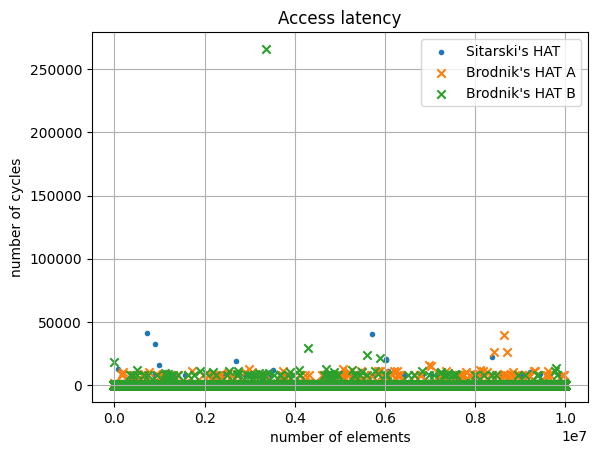
\includegraphics{graphics/hat_access.png}
    \end{center}
    which show how the access time for all 3 HATs looks relatively constant (except that Brodnik's HAT A access is not constant in theory, but is low enough to look like so).

    \subsubsection*{Scan throughput}
    1000 elements are appended and all the 1000 elements are accessed. The total time used to access all elements is measured and we do this for 1000 times.
    Here are the statistics.
    \begin{center}
        \begin{tabular}{|c|c|c|c|}\hline
        & Sitarski's HAT & Brodnik's HAT A & Brodnik's HAT B\\\hline
        mean &  16439.928 & 38772.878 & 53974.224\\\hline
        standard deviation & 1509.39901776038  & 3611.297266234946 & 2422.0789396351224\\\hline
        \end{tabular}
    \end{center}
    For scan throughput, ranking from best to worst is Sitarski's HAT, Brodnik's A, and Brodnik's B.
    Again similar to our access time, Sitarski's HAT perform the best. Brodnik's HAT A beat Brodnik's HAT B this time which is a
    surprise. Even though the access time for Brodnik's HAT A is not constant, but it is still relatively very low
    so it might also occur that Brodnik's HAT B access time get out performed by Brodnik's HAT A because of overhead.

    In term of theory, Sitarski follows the theoretical running time very well with constant low access time (because of simple bitwise).
    But for Brodnik's HAT A, even though in theory, we would say that it is worse than Brodnik's HAT B, but our results has shown that it can be better.

    Of course, it might also means that our Brodnik's HAT B is not optimized enough and we may have to do additional book keeping to make this more optimized.
    Another factor can also stem from the fact that our implementation is a bit different from that of the paper, in this case we might as well trying to find a better
    a better and faster way to compute the number of data blocks before a given superblock.

    \subsubsection*{Overall throughput}
    1000 elements are appended. The total time used to append all 1000 elements is measured and we do this for 1000 times.
    Here are the statistics
    \begin{center}
        \begin{tabular}{|c|c|c|c|}\hline
        & Sitarski's HAT & Brodnik's HAT A & Brodnik's HAT B\\\hline
        mean &  31624.766 & 26366.932 & 28797.736\\\hline
        standard deviation & 1774.3194777840883  & 1691.4454491280528 & 2090.277559154286\\\hline
        \end{tabular}
    \end{center}
    For overall throughput, ranking from best to worst is Brodnik's HAT A, Brodnik's HAT B, and Sitarski's HAT.
    All three HATs does not have that far off running time in terms of mean and they have relatively the same standard deviation.

    This is according to the theory since all of the have $O(1)$ append time (Sitarski's is amortized), the overall throughput
    average out some bad running time for Sitarski's HAT, but still it cannot beat Brodnik's HAT A and B since both of these are constant worst case append time.


    \subsection*{Hash table}
    The test case are seperate into two sections.
    The test case where there is no collision, to just test the implementation.
    And the test case where the collision during insertion happened. To test the collision resolution scheme and how it affects the performance
    The methods and keywords glossary will be describe below:
    \begin{itemize}
        \item size - The size of the initial hash table.
        It's also the number of the element that would (eventually) be in the table
        \item insert - The method insert inserts elements to fill up the table to the brim.
        When it's in the context of collision case, it's an re-insertion of the element in attempt to collide with all index of table.
        (Note: the implementation of cuckoo hashing use simple hash function randomization)
        \item Search - The method search retrieve all the inserted elements sequentially.
        Does not try to search the key that wasn't inserted.
        In the context of collision case, it search for every key again after the collision occurs
        \item Delete - The method delete remove the key that is in the table.
        Does not try to delete the key that wasn't inserted.
        In the context of collision case, it deletes every element in the table after the collision insertion happened.
        \item Scan - The method scan sequentially access all the key in the table.
        In the context of collision case, it scans through the table just like normal, but with maybe new value after collision
    \end{itemize}

    Note: The numbers on the table are in the unit of cpu cycles.
    To convert it to seconds, divide those numbers by 2.6 GHz

    \subsubsection*{No collision case}
    \textbf{Chaining scheme}
    \begin{center}
        \begin{tabular}{|c|c|c|c|c|}\hline
        & Insert & Search & Delete & Scan\\\hline
        size: 1 & 930 & 320 & 3,486 & 670\\\hline
        size: 100 & 143,110 & 13,354 & 40,620 & 26,080\\\hline
        size: 100K & 134,573,520 & 12,750,922 & 38,332,107 & 24,604,098\\\hline
        size: 10M & 14,144,086,730 & 1,319,286,013 & 4,042,035,833 & 2,517,830,762\\\hline
        \end{tabular}
    \end{center}

    For Chaining scheme, the theoretical time for all operations largely depends on the length of the chains on each indexes.
    The expected chains length is $O\left(\dfrac{n}{m}\right)$ where $n$ is the number of keys and $m$ is the number of slots.
    The maximum number of chains is $O\left(\dfrac{\log(n)}{\log(\log(n))}\right)$ where $n$, again, is the number of keys.
    Looking at the table, we see that as the runtime grows proportionally to the size, at the almost the same rate on how the size grows.
    The most notable thing are that:
    \begin{itemize}
        \item Insert method comes at the last place out of the three schemes.
        Weirdly it made a huge jump on the runtime from size of one to size of one-hundred.
        Most likely due the high amount of time of resizing, due to resize factor being multiple of two
        \item Search method comes at the second place.
        This is most like due to the algorithms being un-optimize, as the hash function is called twice during the search
        \item Detele method took the longest out of the three schemes.
        Most likely due to freeing the LinkedList structure
        \item Scan method took the longest compared to other two schemes.
        Since we're keeping the elements as a linked list.
        Extra time to fetch-execute cycle.
    \end{itemize}

    \textbf{Open Addressing scheme}
    \begin{center}
        \begin{tabular}{|c|c|c|c|c|}\hline
        & Insert & Search & Delete & Scan\\\hline
        size: 1 & 3,654 & 380 & 330 & 104\\\hline
        size: 100 & 61,856 & 24,550 & 24,982 & 836\\\hline
        size: 100K & 54,732,644 & 24,174,556 & 26,079,140 & 684,162\\\hline
        size: 10M & 5,143,961,418 & 2,280,300,642 & 2,400,285,752 & 67,605,464\\\hline
        \end{tabular}
    \end{center}

    In Open Addressing scheme, the theoretical time depends on how good the hash function is.
    If the hash function keeps hashing the new key to already occupied index, then the code will take longer to do the operations.
    So the runtime is proportional the number of (linear) probing.
    The most notable thing are that:
    \begin{itemize}
        \item Insert method is the slowest at the start out of the three scheme, but it scales better than chaining, placing it as number two out of the three scheme.
        This is most likely due to implementation design, as an enums were kept for other methods usage
        \item Search method comes at the last place.
        This is most like due to the algorithms being un-optimize, as the hash function is called twice during the search
        \item Detele method placed second out of the three schemes.
        Expectedly should be placed first, due to usage of enums.
        If we were to remove element, it will just be marked empty.
        So the bottleneck is most likely the fact that the hash function was called twice to find the key
        \item Scan method placed first.
        Yay
    \end{itemize}

    \textbf{Cuckoo Hashing scheme}
    \begin{center}
        \begin{tabular}{|c|c|c|c|c|}\hline
        & Insert & Search & Delete & Scan\\\hline
        size: 1 & 158 & 186 & 114 & 556\\\hline
        size: 100 & 8,548 & 5,566 & 6,712 & 9,210\\\hline
        size: 100K & 8,384,710 & 6,419,210 & 7,441,992 & 10,242,288\\\hline
        size: 10M & 656,286,450 & 450,796,896 & 595,650,074 & 918,961,414\\\hline
        \end{tabular}
    \end{center}

    In Cuckoo Hashing scheme, the theoretical time are:
    \begin{itemize}
        \item Insert - $E[O(1)]$
        \item Search - $O(1)$ worst case
        \item Detele - $E[O(1)]$
        \item Scan - $O(n)$ on average
    \end{itemize}
    The most notable thing are that:
    \begin{itemize}
        \item Insert method is the fastest.
        \item Search method comes at the first place.
        \item Detele method placed first
        \item Scan method placed second.
        This is most likely due to maintaining two hash tables.
    \end{itemize}
    The three methods Insert, Search and Delete should have similar runtime like open addressing (since cuckoo hashing is a type of open addressing method).
    But the reason that the results comes about is most likely due to less bottleneck unlike open addressing scheme.

    \subsubsection*{Collision for each and every insert}
    \textbf{Chaining scheme}
    \begin{center}
        \begin{tabular}{|c|c|c|c|c|}\hline
        & Insert & Search & Delete & Scan\\\hline
        size: 1 & 6,436 & 618 & 1,818 & 942\\\hline
        size: 100 & 12,638 & 12,444 & 36,630 & 23,882\\\hline
        size: 100K & 12,805,934 & 12,400,152 & 36,475,868 & 23,906,203\\\hline
        size: 10M & 1,381,820,700 & 1,278,416,286 & 3,839,070,001 & 2,430,914,352\\\hline
        \end{tabular}
    \end{center}
    The most notable thing are that:
    \begin{itemize}
        \item Insert method is the fastest out of the three scheme.
        Since you can just keep connecting the linked list node
        \item Search method comes at the second place.
        This theoretically should be slower than open addressing on worst case scenario.
        But practically, time spent probing took longer than just find the linked list.
        \item Detele method placed last out of the three schemes.
        Since we have to go through linked list to delete it.
        And then we have to reorganize the linked list as well
        \item Scan method placed last.
        Because this is resizable, It has $n$ elements to go through (which include null indexes as well), plus the linked list in each indexes.
    \end{itemize}
    For chaining, this approach sounds very memory expensive.
    Since the pointer to each linked list needs to be remembered.


    \textbf{Open Addressing scheme}
    \begin{center}
        \begin{tabular}{|c|c|c|c|c|}\hline
        & Insert & Search & Delete & Scan\\\hline
        size: 1 & 2,602 & 514 & 354 & 120\\\hline
        size: 100 & 23,580 & 21,490 & 22,120 & 814\\\hline
        size: 100K & 24,796,556 & 22,563,490 & 23,658,006 & 666,302\\\hline
        size: 10M & 2,474,628,412 & 2,260,518,832 & 2,360,901,784 & 66,875,470\\\hline
        \end{tabular}
    \end{center}
    The most notable thing are that:
    \begin{itemize}
        \item Insert method is the slowest.
        \item Search method comes at the last place.
        \item Delete method placed second.
        \item Scan method placed first.
    \end{itemize}
    The more the probing, the longer the operations.
    This applies to Insert, Search and Delete

    \textbf{Cuckoo Hashing scheme}
    \begin{center}
        \begin{tabular}{|c|c|c|c|c|}\hline
        & Insert & Search & Delete & Scan\\\hline
        size: 1 & 346 & 208 & 172 & 556\\\hline
        size: 100 & 183,484 & 8,524 & 8,986 & 9,048\\\hline
        size: 100K & 107,326,484 & 9,201,168 & 8,696,178 & 9,369,126\\\hline
        size: 10M & 1,572,211,006 & 513,099,226 & 598,603,314 & 921,694,710\\\hline
        \end{tabular}
    \end{center}
    The most notable thing are that:
    \begin{itemize}
        \item Insert method is the second fastest.
        \item Search method comes at the first place.
        \item Delete method placed first.
        \item Scan method placed second.
        \item Notice that collision, the load on insert highly increases, but at a trade for faster search and delete comparing to other scheme
    \end{itemize}

    From the looks of it, Cuckoo Hashing seems to be the most generally speedy collision resolution scheme for hash table.
    However, further testing/test cases needed to be done.
    As well as the optimization for all the scheme for a fairer test.

    \section*{Conclusion}
    We have implemented and benchmark 3 versions of HATs and 3 versions of hash table.

    For HATs, we have found that Brodnik's HAT A and B does very well for append/overall throughput when compare to Sitarski's HAT this is partly due to
    the background-rebuilding optimization that has been implement for both of the former and the fact that the former does not copy over all the elements
    when expanding. For access/scan throughput, Sitarski's outperformed Brodnik's HAT A and B, this is because the former does only simple bitwise operation to figure out the index,
    but Brodnik's HAT A is more complex which involves square root which does not run in constant time and Brodnik's HAT B even though use some bitwise operation and BSR x86 assembly directly, but
    the arithmetics required can be heavy enough to weight it down, additional book keeping might be needed to make this better. Also noted that the modification from
    the original paper for the function used to access might also affect the running time.

    Also note that Brodnik's HAT A performed better than Brodnik's HAT B for scan throughput, even though Brodnik's HAT B promise better theoretical constant running time, but in this
    case our implementation might introduce some overhead to make this worse than the Brodnik's HAT A which does not have constant access, but access time can be low enough to beat the overhead for
    Brodnik's HAT B. This does show that even though the theory says that Brodnik's HAT B is better than Brodnik's HAT A, but our result show that this is not the case in practice.
    If we are taking in to account the ease of implementation for Brodnik's HAT A and our results for its performence, Brodnik's HAT A is better than Brodnik's HAT B in this case.

    For Hash tables' collision scheme, we've look over how each of the hashing scheme are compared to each other in a non-collision case and full collision case.
    In general the cuckoo hashing scheme seems to be very well rounded, placing generally first in both categories.
\end{document}
